\documentclass[aspectratio=169]{beamer}

\usetheme{Madrid}
\usecolortheme{seahorse}
\usepackage[utf8]{inputenc}
\usepackage[T1]{fontenc}
\usepackage[serbian]{babel}
\usepackage{graphicx}
\usepackage{booktabs}

\title[Detekcija vozila pomo\'cu KNM]{Detekcija vozila na slikama pomo\'cu\\konvolucionih neuronskih mre\v za}
\author{Aleksa Vukadinovi\'c}
\institute{Ra\v cunarska inteligencija}
\date{\today}

\begin{document}

% ---- Slajd 1: Naslov ----
\begin{frame}
  \titlepage
\end{frame}

% ---- Slajd 2: Sadr\v zaj ----
\begin{frame}{Sadr\v zaj}
  \tableofcontents
\end{frame}

\section{Problem}
% ---- Slajd 3: Problem ----
\begin{frame}{Problem: detekcija vozila}
  \begin{itemize}
    \item \textbf{Cilj:} odlu\v citi da li slika sadr\v zi \emph{vozilo}.
    \item Osnovni gradivni blok sistema za nadzor saobra\'caja i percepciju u
          autonomnoj vo\v znji.
    \item Formalno, u\v cimo
          $f_\theta : \mathbb{R}^{3\times 32\times 32} \to \{0,1\}$
          \\($1$ = vozilo, $0$ = nije vozilo).
    \item Tretiramo ga kao \textbf{binarnu klasifikaciju slika} -- klasifikator
          na kome se grade detektori (Faster R-CNN, YOLO).
  \end{itemize}
\end{frame}

\section{Pregled literature}
% ---- Slajd 4: Srodni radovi ----
\begin{frame}{Nau\v cna pozadina}
  \begin{itemize}
    \item \textbf{LeNet} (LeCun i sar., 1998) -- prva obu\v civa KNM.
    \item \textbf{AlexNet} (Krizhevsky i sar., 2012) -- duboke KNM nadma\v suju
          ru\v cno konstruisana obele\v zja (npr.\ HOG).
    \item \textbf{VGG} (Simonyan i Zisserman, 2015) -- nizovi malih $3\times3$
          konvolucija. \emph{(arhitektura koju reprodukujemo)}
    \item \textbf{ResNet} (He i sar., 2016) -- rezidualne veze.
    \item Klju\v cne tehnike: BatchNorm, Dropout, Adam/AdamW, kosinusni
          raspore\dj iva\v c stope u\v cenja.
  \end{itemize}
  \vfill
  \footnotesize Ovaj projekat \textbf{reprodukuje} utemeljenu metodologiju; nije
  re\v c o novoj arhitekturi.
\end{frame}

\section{Metoda}
% ---- Slajd 5: Skup podataka ----
\begin{frame}{Skup podataka: CIFAR-10 $\rightarrow$ binarni}
  \begin{columns}
    \begin{column}{0.55\textwidth}
      \begin{itemize}
        \item CIFAR-10: $60{,}000$ slika, $32\times32$, 10 klasa.
        \item Preslikano u binarni cilj:
      \end{itemize}
      \medskip
      \begin{tabular}{ll}
        \toprule
        \textbf{Cilj} & \textbf{Klase} \\
        \midrule
        vozilo (1)      & avion, automobil, \\ & brod, kamion \\
        nije vozilo (0) & ptica, ma\v cka, jelen, \\ & pas, \v zaba, konj \\
        \bottomrule
      \end{tabular}
    \end{column}
    \begin{column}{0.45\textwidth}
      \begin{itemize}
        \item $50$k trening / $10$k test.
        \item Trening deo $90/10$ za validaciju.
        \item Augmentacija: nasumi\v cno ise\-canje + horizontalno
              preslikavanje.
        \item Normalizacija po kanalima.
      \end{itemize}
    \end{column}
  \end{columns}
\end{frame}

% ---- Slajd 6: Arhitektura ----
\begin{frame}{Arhitektura: VehicleCNN}
  \begin{columns}
    \begin{column}{0.5\textwidth}
      \footnotesize
      \begin{tabular}{ll}
        \toprule
        \textbf{Sloj} & \textbf{Izlaz} \\
        \midrule
        Ulaz             & $3\times32\times32$ \\
        ConvBlock(64)    & $64\times16\times16$ \\
        ConvBlock(128)   & $128\times8\times8$ \\
        ConvBlock(256)   & $256\times4\times4$ \\
        Glob.\ usredn.   & $256$ \\
        Dropout-FC(128)  & $128$ \\
        Dropout-FC(2)    & $2$ (logiti) \\
        \bottomrule
      \end{tabular}
    \end{column}
    \begin{column}{0.5\textwidth}
      \begin{itemize}
        \item ConvBlock = 2$\times$(Conv $3\times3$ -- BN -- ReLU) + MaxPool.
        \item $\sim$1.18M parametara.
        \item Gubitak: unakrsna entropija.
        \item Optimizator: AdamW, lr $10^{-3}$.
        \item Kosinusni raspore\dj iva\v c, 20 epoha.
      \end{itemize}
    \end{column}
  \end{columns}
\end{frame}

% ---- Slajd 7: Referentne metode ----
\begin{frame}{Referentne metode za pore\dj enje}
  Razvili smo dve jednostavnije metode na sirovim pikselima da izolujemo
  vrednost konvolucija:
  \begin{itemize}
    \item \textbf{Logisti\v cka regresija} -- linearni klasifikator (donja
          granica).
    \item \textbf{MLP (bez konvolucija)} -- potpuno povezan $(256,128)$;
          nelinearan ali bez deljenja te\v zina / prostorne lokalnosti.
  \end{itemize}
  \vfill
  Pore\dj enje KNM naspram MLP pokazuje ta\v cno koliko \emph{konvoluciona
  struktura} doprinosi.
\end{frame}

\section{Rezultati}
% ---- Slajd 8: Krive treniranja ----
\begin{frame}{Dinamika treniranja}
  \centering
  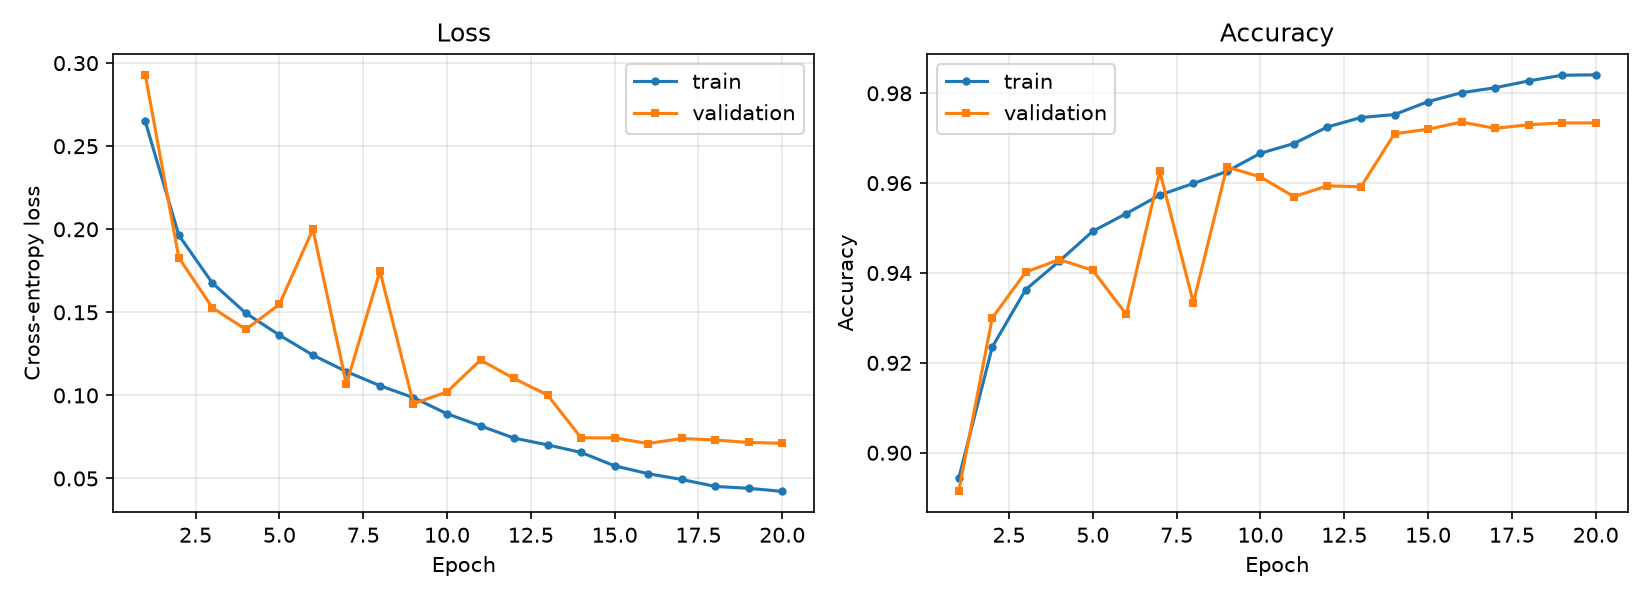
\includegraphics[width=0.95\textwidth]{../reports/figures/training_curves.png}
  \\[0.3em]
  \footnotesize Najbolja validaciona ta\v cnost $97.36\%$ u epohi 16; stabilan
  razmak trening/validacija $\Rightarrow$ nema ozbiljnog preprilago\dj avanja.
\end{frame}

% ---- Slajd 9: Tabela pore\dj enja ----
\begin{frame}{Kvantitativno pore\dj enje (test skup)}
  \centering
  \begin{tabular}{lccccc}
    \toprule
    \textbf{Model} & \textbf{Ta\v c.} & \textbf{Prec.} & \textbf{Odz.} & \textbf{$F_1$} & \textbf{AUC} \\
    \midrule
    Logisti\v cka regresija    & 0.816 & 0.791 & 0.733 & 0.761 & 0.879 \\
    MLP (bez konv.)           & 0.880 & 0.854 & 0.845 & 0.850 & 0.943 \\
    \textbf{VehicleCNN (na\v se)} & \textbf{0.973} & \textbf{0.969} & \textbf{0.963} & \textbf{0.966} & \textbf{0.997} \\
    \bottomrule
  \end{tabular}
  \vfill
  \begin{itemize}
    \item Linearno $\to$ MLP: $+6.5$ p.p.\ (nelinearnost).
    \item MLP $\to$ KNM: $+9.2$ p.p.\ (\textbf{konvolucije}).
  \end{itemize}
\end{frame}

% ---- Slajd 10: Dijagnostika ----
\begin{frame}{Analiza gre\v saka}
  \centering
  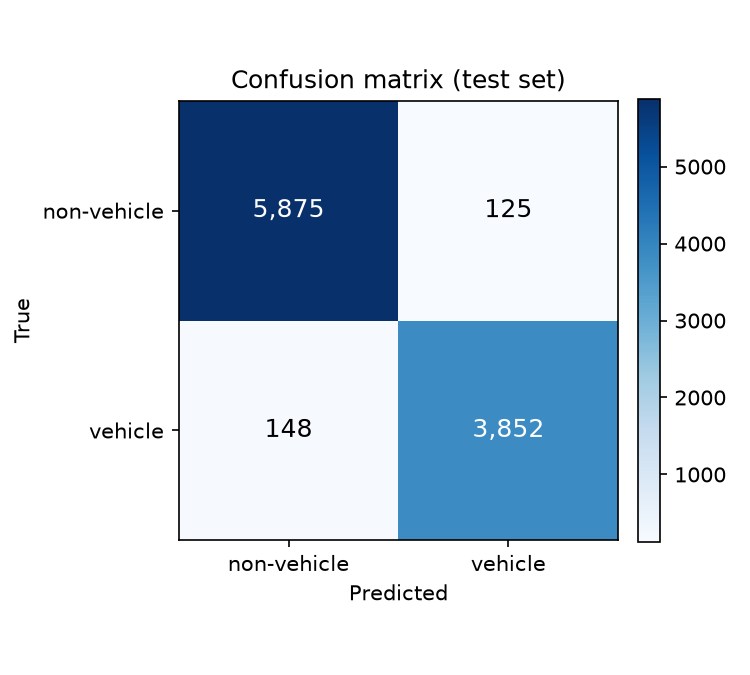
\includegraphics[width=0.32\textwidth]{../reports/figures/confusion_matrix.png}
  \hfill
  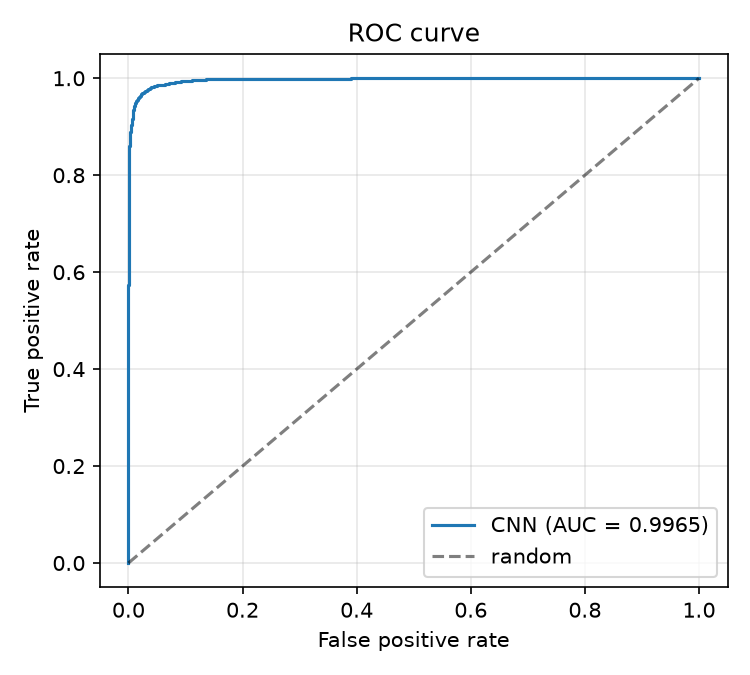
\includegraphics[width=0.32\textwidth]{../reports/figures/roc_curve.png}
  \hfill
  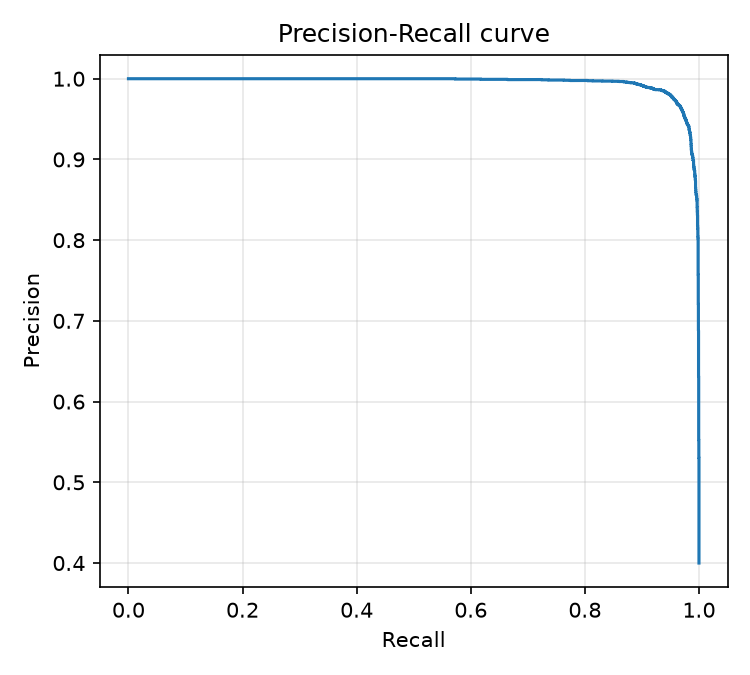
\includegraphics[width=0.32\textwidth]{../reports/figures/pr_curve.png}
  \\[0.3em]
  \footnotesize Uravnote\v zene gre\v ske; preciznost $0.969$ $\approx$ odziv
  $0.963$; ROC-AUC $0.9965$.
\end{frame}

% ---- Slajd 11: Kvalitativni rezultati ----
\begin{frame}{Kvalitativni rezultati na jednostavnim primerima}
  \centering
  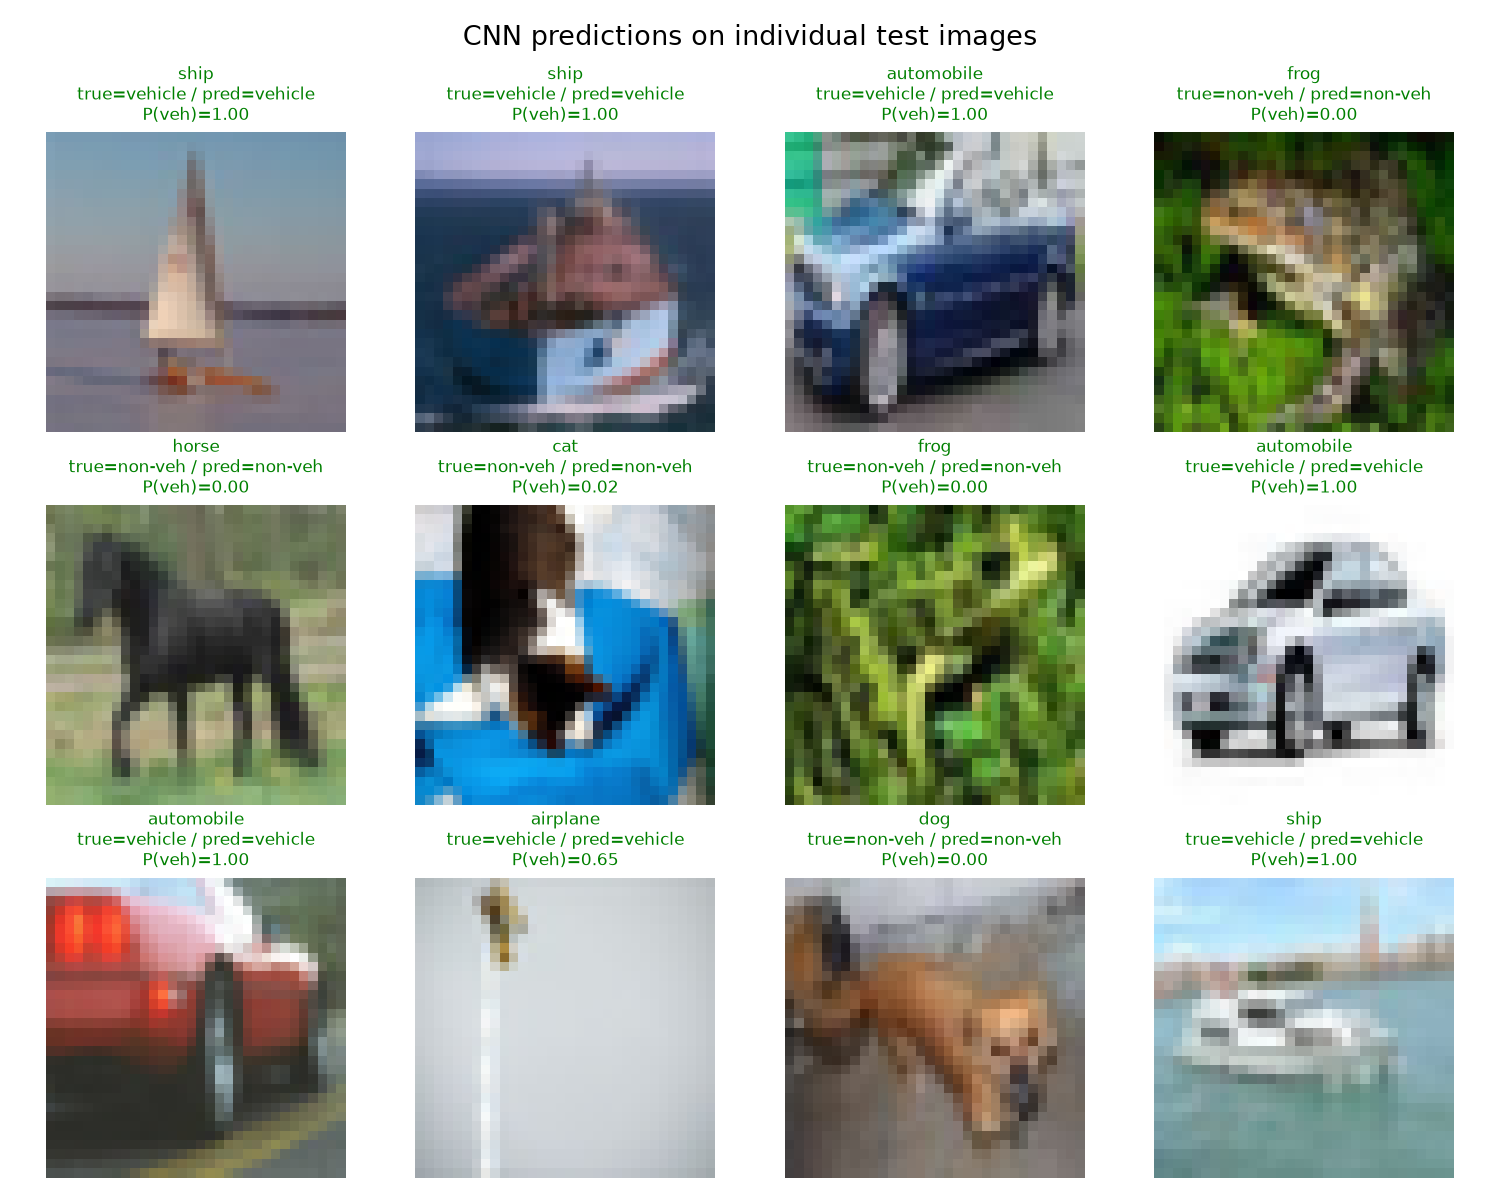
\includegraphics[width=0.72\textwidth]{../reports/figures/sample_predictions.png}
  \\[0.2em]
  \footnotesize Pouzdan na jasnim primerima; razumno ni\v za pouzdanost na
  netipi\v cnim prikazima (zeleno = ta\v cno).
\end{frame}

% ---- Slajd 12: Okru\v zenje ----
\begin{frame}{Eksperimentalno okru\v zenje}
  \begin{itemize}
    \item \textbf{Hardver:} Apple M4 Pro (14 jezgara), 48~GB RAM.
    \item \textbf{Akcelerator:} Apple MPS (podr\v zava i CUDA / procesor).
    \item \textbf{OS:} macOS 26.5.1 (arm64).
    \item \textbf{Softver:} Python 3.11, PyTorch 2.12, torchvision 0.27,
          scikit-learn 1.9.
    \item \textbf{Vreme treniranja:} KNM $\approx 4.3$ min ($\sim$12.7\,s/epohi);
          referentne metode $1.5$\,s / $8.3$\,s.
  \end{itemize}
\end{frame}

\section{Zaklju\v cak}
% ---- Slajd 13: Zaklju\v cak ----
\begin{frame}{Zaklju\v cak i dalji rad}
  \textbf{Zaklju\v cak}
  \begin{itemize}
    \item Kompaktna KNM posti\v ze ta\v cnost $97.3\%$, AUC $0.997$.
    \item Jasno nadma\v suje samostalno razvijene linearnu i MLP metodu.
    \item Konvolucije su presudni \v cinilac.
  \end{itemize}
  \textbf{Dalji rad}
  \begin{itemize}
    \item Potpuna \emph{detekcija} sa grani\v cnim okvirima (Faster R-CNN / YOLO).
    \item Slike saobra\'caja vi\v se rezolucije iz stvarnog sveta.
    \item Sna\v znije osnove (ResNet); fini tipovi vozila.
  \end{itemize}
\end{frame}

% ---- Slajd 14: Demonstracija ----
\begin{frame}{Demonstracija rada}
  \centering
  \Large Demonstracija skripte \texttt{predict.py}
  \vfill
  \normalsize
  \texttt{python predict.py --image putanja/do/slike.jpg}
  \vfill
  \footnotesize Izlaz: \texttt{VEHICLE / NOT A VEHICLE} sa
  $P(\text{vozilo})$.
\end{frame}

% ---- Slajd 15: Hvala ----
\begin{frame}{Hvala}
  \centering
  \Large Pitanja?
  \vfill
  \normalsize Kod, dokumentacija i slike dostupni su u javnom GitHub
  repozitorijumu.
\end{frame}

\end{document}
